\chapter{Background}
\section{Handover}
Handover is the process in which an active cell connection (data or cellular) is transferred from a source base station to a target station. This is done to maintain continuous connectivity for mobile devices. Handover is a crucial technique in radio communication networks for both mobility management and load balancing.

A UE \footnote{User Equipment - any device that can connect to a cell network, for instance a mobile phone} will have an active connection to a single base station (BS) at one time, with its signal strength being measured by the UE in terms of its Received Signal Reference Power (RSRP) \ab{explain that RSRP is used to trigger handover}. RSRP can be affected by a number of different factors, but the two main influences are the distance to the base station (as propagation loss is logarithmically proportional to distance), and line of sight (LOS) blockages (as direct waves have higher power than reflected waves). 
RSRP is correlated with data throughput, and with the goal of maximising Quality of Services (QoS), we want to maximise RSRP. A cell connection will also become unstable and/or drop at low RSRP strength.

\subsection{Handover Procedure}
\begin{enumerate}
    \item A UE will measure the RSRP of all BSs in range, and send the report to the connected (source) BS.
    \item The source BS will compare the measured RSRP metrics, and decide whether to initiate handover. This decision is made with various algorithms discussed in \ref{sec:algorithms}, but all focus on maximising the UE's QoS by handing the connection over to a BS with a higher RSRP.
    \item If the BS decides to initiate handover, it will determine which neighbouring BS to transfer the connection to. There are various protocols that determine the manner in which a connection is transferred, however this is outside of this paper's scope. Regardless of the protocol used, there will be a drop in connectivity and/or throughput.
    \item The connection between a UE and the source BS can drop if handover is not triggered before the RSRP drops below a level where communication is possible. This is termed Handover Failure (HOF), and has a much greater impact on connectivity, as so must be minimised.
    \item Handover decisions are not always optimal; a UE transferred to a neighbouring BS could be transferred back to the source BS if the RSRP values are not stable. This results in two unneeded handovers, decreasing QoS as well as increasing server load. This is termed Handover Ping Pong (HOPP) as must be minimised.
\end{enumerate}

\subsection{Indoor Environments}
The challenge of handover is relatively simple in outdoor environments, and with it being the main target of literature on the subject, there exist many solutions to its various challenges. 5G however will be ubiquitously deployed in indoor environments. The indoor wireless channel is much harder to model, as LOS blockages are much more common due to the constrained environment. Furthermore, indoor deployments lend themselves towards much smaller cells (the area a BS serves), and therefore handovers will occur much more frequently as cell density increases.

The main motivation and focus of this paper therefore is on the understanding, modelling and prediction of handover in indoor environments \ab{to keep a level of connection quality}.


% \section{Challenges}
% \subsection{Mobility Management}
% Mobility Management is an integral part of a cellular network, and ensures UEs maintain a good quality connection to the network. UEs, as mobile devices, do not remain stationary, and will move through different cells as a person walks, moves or drives. The Mobility Management Unit (MMU) will transfer the connection of the device between different station through the use of handover. As and when to initiate handover is a very broad topic with hundreds of research papers dedicated to optimising various parameters and metrics, and is not a simple decision. Premature handover can lead to a phenomenon termed Handover Ping Pong (HOPP) where a UE is transferred back to the source cell in a short period of time, thereby having needlessly interrupted the UEs cell connection twice, as well as increasing the server load. Late handover can lead to a cell experiencing much lower data throughput, or disconnecting entirely from the network (Handover Failure, HOF).

% A key difficulty therefore can come from fast-moving users, as handovers must be performed much faster.

% \subsection{Load Balancing}
% Another key factor to consider is Load Balancing in a cellular network. Active cell connections require a certain amount of hardware resources, and therefore to maintain good performance across the network, handovers should not just be employed for mobility management, but also for equitable distribution of traffic across base stations. This ensures efficient resource utilisation and reduces congestion. A careful balance must be struck to offset individual UE performance with average network performance using handovers.

\section{Handover Algorithms}
\label{sec:algorithms}
The focus of this paper is to understand the effects of handover and to design and test various strategies to minimise the negative effects. We therefore need to understand the various methods used to initiate handover and classify the various algorithms.

\subsection{Classical Approach}

\begin{wrapfigure}[18]{r}{0.5\textwidth}
    % \centering
     \raisebox{0pt}[\dimexpr\height-2\baselineskip\relax]{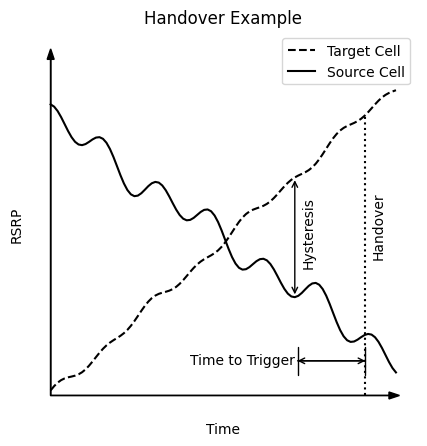
\includegraphics[width=0.48\textwidth]{src/img/hysteresis_ttt.png}}
    % 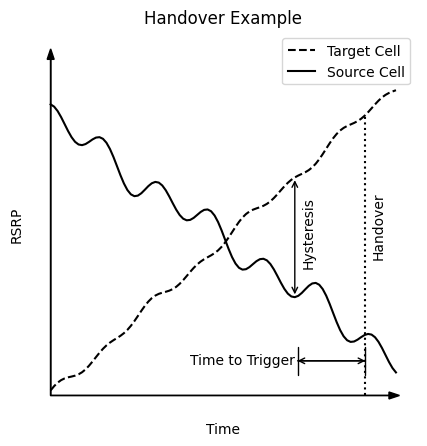
\includegraphics[width=0.48\textwidth]{src/img/hysteresis_ttt.png}
    \caption{Handover based on Hysteresis and TTT}
    \label{fig:hysteresis_handover}
\end{wrapfigure}

The standard approach taken towards handover uses two parameters, \textit{Hysteresis} and \textit{Time to Trigger}, to determine when to trigger handover. When a neighbour cell has an RSRP greater than the current cell by a set margin, i.e. the hysteresis, for a given period of time, i.e. time to trigger, the handover is triggered and the UE is transferred to the neighbour cell. This process is illustrated in Figure \ref{fig:hysteresis_handover}. Alternative heuristics are often needed, as the standard approach is not robust enough for dynamic environments.



\clearpage %============================= CLEAR PAGE  =====================================%

\subsection{Alternative Heuristics}
Using the relative RSRPs (such as Hysteresis), with some delay (such as Time to Trigger) form the basis of the majority of existing handover algorithms. Other parameters are suggested and modelled in literature are throughput, location, load balancing, user’s velocity, service delay, and distance. \cite{nyangaresi_efficient_2022}.

\citet{hatipoglu_handover-based_2020} presented a handover-based load balancing algorithm for HetNets. The paper utilised UE speeds in determining handover, an metric which is unrealistic to obtain in practice. The algorithm itself is fairly simplistic, and while the paper showed good results, the algorithm does not consider key metrics such as RSRP, or connection speed.

\subsection{Machine Learning}
Seeing handover as an optimisation problem, the utilisation of Machine Learning (ML) in the problem of handover is a natural one. For this reason, ML techniques are appealing to provide better performance than the more naive algorithms. As ML techniques do not require a model of the environment, this is especially applicable to indoor environments, where modelling proves difficult.

ML algorithms can be subdivided into supervised, unsupervised and reinforcement learning. Supervised and unsupervised algorithms perform either regression or classification on a set of inputs. Reinforcement learning is based on the concept that the algorithm will learn to maximise its rewards in a given environment through learning the optimal policy. The optimal policy in our case is a sequence of handover decisions that maximise throughput while minimising HOF and HOPP. The use of reinforcement learning has been surveyed in \cite{mollel_survey_2021}.

Reinforcement learning is a broad grouping of algorithms. This includes Multi-Armed Bandits, Monte Carlo methods, Q-learning and Deep Q-learning.

\citet{yajnanarayana_5g_2020} presented a handover algorithm using Contextual Multi-Armed Bandit reinforcement learning. This ML model provided modest improvements (0.3dB) in the average RSRP of devices. The authors also wrote their own network simulator, one which used sophisticated propagation models, such as log-shadowing, as well as the WINNER UMa Model. The code used to simulate it was not released, however, providing very little reproducibility of the paper. The improvements were relatively minor, and better results could possibly be obtained with a deep-learning based Reinforcement model

\citet{mollel_survey_2021} further introduces and surveys an alternative method of using machine learning. The pure network-based models operate only on radio data, such as RSRP and base station states, however, an alternative heuristic uses optical information, such as camera feeds to better predict handover. This is done through tracking UE movement through object detection, and predicting when LOS will be obstructed. While this is a tool that can prove very useful, it introduces many limitations as the models trained will be very location-dependent, and have the greatest impact in indoor environments due to the greater LOS blockage rate.

\section{Handover Testbeds}
To evaluate experimental algorithms, we need some way to emulate a network. Many authors choose to run custom simulations using propagation algorithms to model path loss and simulate the network devices. A much better method is to use a software radio suite as a testbed. This allows us to emulate UEs, base stations (BSs), and the core network (CN).

There are a few options available for use, with the major software being srsRAN, OpenAirInterface and Aether. For this paper, srsRAN is chosen due to its clear open source code, and extensive tutorials to get started with. While a fully custom testbed allows for greater flexibility, the realistic nature of using software radio suites will give results that much better reflect how the algorithms would perform in a real-world scenario, and so arguably give more useful results.

\citet{powell_handover_2021} presented a testing framework for 4G experiments using srsRAN and performed basic experiments with it. The framework was presented clearly, and I was able to replicate the results of their simulation. The experiments they performed however were limited as signal strength was arbitrarily introduced by attenuating a signal, and did not utilise signal propagation algorithms.


\section{Previous Work}
\citet{}
\ab{Include papers that model and/or measure the negative impact of handover in indoor scenarios, whether is simulation or real-world analysis.}

\section{Research Gap}
\begin{itemize}
    \item Load Balancing in realistic testbed
    \item Improve LB with better heuristics
\end{itemize}

\section{Other points}
\begin{itemize}
    \item Reactive vs Predictive
    \item Use SINR for HO params
    \item Spikes in traffic due to events, past data
    \item Colloseun Emulator
    \item O-RAN
\end{itemize}